\ifdefined\COMPLETE
\else
    \input{./preambule-sacha-utf8.ltx}
    \begin{document}
\fi


\section{Repères du plan}

\subsection{Définition}

Soit O un point.

Soient $\vec{i}$ et $\vec{j}$ deux vecteurs non colinéaires.

% Les petits poids 
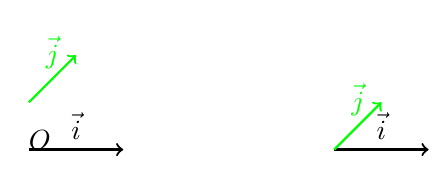
\begin{tikzpicture}[scale=0.6]

\draw[thick, ->] (0,0)  --  node[midway,above]{$\vec{i}$}(2,0) ;
\draw[color=green, thick, ->] (0,1)  --  node[midway,above]{$\vec{j}$}(1,2) ;
\tkzDefPoint [label=below left:$O$](6,0){O}
\tkzDrawPoint [color=black,size=5](O)

\draw[thick, ->] (6,0)  --  node[midway,above]{$\vec{i}$}(8,0) ;
\draw[color=green, thick, ->] (6,0)  --  node[midway,above]{$\vec{j}$}(7,1) ;

\end{tikzpicture}

$\left(O, \vec{i}, \vec{J}\right)$ est un repère du plan.

\subsection{Coordonnées d'un point dans un repère}

Soit $\left(O, \vec{i}, \vec{j}\right)$\\

Soit M un point. \\

Il existe un nombre réel x unique et un nombre réel y unique tels que : \\

$ \overrightarrow{OM} = x\vec{i} + y\vec{j} $ \\

On écrit :

\begin{itemize}
\item $x$ est l'abscisse de M dans $\left(O, \vec{i}, \vec{j}\right)$\\
\item $y$ est l'ordonnée de M dans $\left(O,\vec{i}, \vec{j}\right)$\\
\end{itemize}

\textbf{Remarque}

On dit que $x$ et $y$ sont les coordonnées de M dans $\left(O, \vec{i}, \vec{j}\right) $\\

% Le repère oblique 
\begin{tikzpicture}[scale=0.5]

\draw[color=black, very thick, ->] (0,0)  --  node[midway,below]{$\vec{i}$}(2,0) ;
\draw[color=black, very thick, ->] (0,0)  --  node[midway,above]{$\vec{j}$}(1,1) ;
\draw[color=black, ->] (-3,0) --( 15,0) ; 
\tkzText(12,-0.3){\textcolor{black}{Axes des abscisses}}
\draw[color=black, ->] (-3,-3) -- ( 10,10) ; 
\tkzText(7,8){\textcolor{black}{Axes des}}
\tkzText(6,7.5){\textcolor{black}{ordonnées}}
\draw[color=black, thick, ->] (0, 0) -- (8, 0) ; 
\tkzText(4, 0){\textcolor{black}{|}} 
\tkzText(6, 0){\textcolor{black}{|}} 

\draw[color=black, thick, ->] (8, 0) -- (11, 3) ; 
\tkzText(2, 2){\textcolor{black}{-}} 
\tkzText(3, 3){\textcolor{black}{-}} 

\draw[color=black, thick, -] (3, 3) -- (11, 3) ; 
\draw[color=red, very thick, ->] (0, 0) -- (11, 3) ; 

\tkzText(11.3,3.3){\textcolor{black}{M}}
\end{tikzpicture}\\

$M\left(x,y,\right) \textrm{dans} \left(O, \vec{i}, \vec{j}\right) \Longleftrightarrow \overrightarrow{OM} = x\vec{i} + y\vec{j} $\\
\newpage 
Dans la pratique, on utilise un repère orthogonal, ou mieux, un repère orthonormal. Avant, on appelait cela un repère "orthonormé".\\

% Repère orthogonal
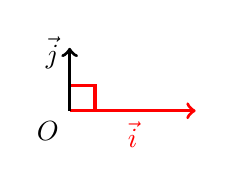
\begin{tikzpicture}[scale=.8]
\tkzInit[xmin=-3,xmax=4, ymin=-2, ymax=4]
\tkzDrawXY [noticks]

\draw[color=red, very thick, ->] (0,0)  --  node[midway,below]{$\vec{i}$}(2,0) ;
\draw [color=red, very thick] (0,.4)  -- (.4,.4) -- (.4, 0) ;  
\draw[color=black, very thick, ->] (0,0) node [below left] {$O$} --  node[midway,above left]{$\vec{j}$}(0,1) ;
\end{tikzpicture} \hspace{1cm}
% Repère orthonormal                 <<<<<<<<<<<<<<<<<<<<<<
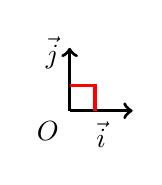
\begin{tikzpicture}[scale=.8]
\tkzInit[xmin=-3,xmax=4, ymin=-2, ymax=4]
\tkzDrawXY [noticks]

\draw[color=black, very thick, ->] (0,0)  --  node[midway,below]{$\vec{i}$}(1,0) ;
\draw[color=black, very thick, ->] (0,0) node [below left] {$O$} --  node[midway,above left]{$\vec{j}$}(0,1) ;
\draw [color=red, very thick] (0,.4)  -- (.4,.4) -- (.4, 0) ;  
\end{tikzpicture}
\newpage 
\subsection{Milieu d'un segment}

Soit $\left(O,\vec{i}, \vec{j}\right)$ un repère.

Soient $A\left(x_A,y_A \right) $ et $B \left( x_B,y_B \right) $. 

Soit I le milieu de $\left[AB\right]$ \\

On a I $ \left(\underbrace{\dfrac{x_A + x_B}{2}}_{\textrm{Moyenne des abscisses}}, \underbrace{\dfrac{y_A + y_B}{2}}_{\textrm{Moyenne des ordonnées}}\right) $ \\

\subsubsection{Exemple}

\begin{tabular}{ll}
$x_I = \dfrac{x_A + x_B}{2} $ & $y_I = \dfrac{y_A + y_B}{2}$ \\
 & \\
$ x_I = \dfrac{-3 + 7}{2}$ & $y_I = \dfrac{2+6}{2}$ \\
 & \\
$x_I = 2$ & $y_I = 4$ \\
\end{tabular}

Donc $I\left(2,4\right)$

\begin{center}
% Milieu d'un segment
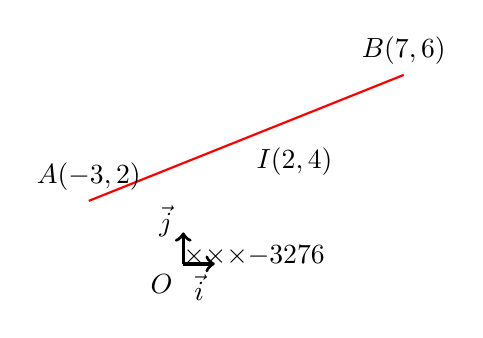
\begin{tikzpicture}[scale=.4]
\tkzInit[xmin=-4,xmax=8, ymin=-4, ymax=10]
\tkzDrawXY [noticks]
\draw[color=black, very thick, ->] (0,0)  --  node[midway,below]{$\vec{i}$}(1,0) ;
\draw[color=black, very thick, ->] (0,0) node [below left] {$O$} --  node[midway,above left]{$\vec{j}$}(0,1) ;

\draw [color=red, thick] (-3,2) node [color=black, above] {$A (-3, 2)$} -- (2,4)
node [color=black, below right] {$I (2, 4)$} -- (7,6)  node [color=black, above] {$B (7, 6)$} ; 
\tkzText(-3,2){\textcolor{black}{$\times$}}
\tkzText(2,4){\textcolor{black}{$\times$}}
\tkzText(7,6){\textcolor{black}{$\times$}}

\tkzDefPoint(-3,0){XA} 
\tkzText(-3,0){\textcolor{black}{|}}
\tkzLabelPoint[color=black,below](XA){$-3$}
\tkzDefPoint(0,2){YA}
\tkzText(0,2){\textcolor{black}{-}}
\tkzLabelPoint[color=black,right](YA){$2$}
\tkzDefPoint(7,0){XB} 
\tkzLabelPoint[color=black,below](7,-.5){$7$}
\tkzText(7,0){\textcolor{black}{|}}
\tkzDefPoint(0,6){YB}
\tkzText(0,6){\textcolor{black}{-}}
\tkzLabelPoint[color=black,right](YB){$6$}

\end{tikzpicture}\\
\end{center}

\subsubsection{Démonstration}

$ \overrightarrow{IA} + \overrightarrow{IB} = \overrightarrow{0} $\\

$ \overrightarrow{IO} + \overrightarrow{OA} + \overrightarrow{IO} + \overrightarrow{OB} = \overrightarrow{0} $\\

$ 2\overrightarrow{IO} = -\overrightarrow{OA} -\overrightarrow{OB} $\\

$ \overrightarrow{IO} = -\dfrac{1}{2} \overrightarrow{OA} - \dfrac{1}{2} \overrightarrow{OB} $\\

$ \overrightarrow{OI} = \dfrac{1}{2} \overrightarrow{OA} + \dfrac{1}{2} \overrightarrow{OB} $\\

$ \overrightarrow{OI} = \dfrac{1}{2} \left(x_A\vec{i} + x_B\vec{j} \right) + \dfrac{1}{2} \left( y_A\vec{i} + y_B\vec{j}\right) $\\

$ \overrightarrow{OI} = \dfrac{x_A + x_B}{2}\vec{i} + \dfrac{y_A + y_B}{2} \vec{j} $


\newpage


\subsection{Centre de gravité d'un triangle}

Soit $\left(O, \vec{i}, \vec{j}\right)$ un repère.

Soient les points :

\begin{itemize}
\item $A\left(x_A,y_A\right)$\\
\item $B\left(x_B,y_B\right)$\\
\item $C\left(x_C,y_C\right)$\\
\end{itemize}
 
 Soit G le centre de gravité de ABC.
 
On a G $ \left(\underbrace{\dfrac{x_A + x_B + x_C}{3}}_{\textrm{Moyenne des abscisses}}, \underbrace{\dfrac{y_A + y_B + y_C}{3}}_{\textrm{Moyenne des ordonnées}}\right) $ \\

\subsubsection{Exemple}

\begin{tabular}{ll}
$x_G = \dfrac{x_A + x_B + x_C}{3} $ & $y_G = \dfrac{y_A + y_B + y_C}{3}$ \\
$ x_G = \dfrac{5 + 1 + 9}{3}$ & $y_G = \dfrac{10 + 2+6}{3}$ \\
$x_G = 5$ & $y_G = 6$ \\
\end{tabular}

Donc $G\left(5,6\right)$\\

% Centre de gravité
\begin{tikzpicture}[scale=.8]
\tkzInit[xmin=-1,xmax=10, ymin=-1, ymax=11]
\tkzDrawXY [noticks]
\draw[color=black, very thick, ->] (0,0)  --  node[midway,below]{$\vec{i}$}(1,0) ;
\draw[color=black, very thick, ->] (0,0) node [below left] {$O$} --  node[midway,above left]{$\vec{j}$}(0,1) ;

\tkzText(1,2){\textcolor{black}{$\times$}}
\tkzText(5,10){\textcolor{black}{$\times$}}
\tkzText(9,6){\textcolor{black}{$\times$}}
\tkzText(5,6){\textcolor{black}{$\times$}}

\tkzDefPoint(5,10){A} 
\tkzDefPoint(1,2){B} 
\tkzDefPoint(9,6){C} 
\tkzDefPoint(5,6){G} 

\tkzText(5,0){\textcolor{black}{|}}
\tkzText(9,0){\textcolor{black}{|}}
\tkzText(0,2){\textcolor{black}{-}}
\tkzText(0,6){\textcolor{black}{-}}
\tkzText(0,10){\textcolor{black}{-}}


\tkzDefPoint(5,0){XA}  \tkzDefPoint(0,10){YA}
\tkzDefPoint(1,0){XB}  \tkzDefPoint(0,2){YB}
\tkzDefPoint(9,0){XC}  \tkzDefPoint(0,6){YC}

\tkzLabelPoint[color=black,below](XA){$5$}
\tkzLabelPoint[color=black,left](YA){$10$}
\tkzLabelPoint[color=black,left](YB){$2$}
\tkzLabelPoint[color=black,below](XC){$9$}
\tkzLabelPoint[color=black,left](YC){$6$}

\draw [color=red, thick] (A)  node [color=black, above ] {$A$} 
-- (B) node  [color=black,below] {$B$}   -- (C) node  [color=black,right] {$C$}   -- cycle ; 

\draw [color=black, dashed] (3,6) -- (9,6) ; 
\draw [color=black, dashed] (5,10) -- (5,4) ; 

\tkzLabelPoint[color=black,above right](G){$G$}

\end{tikzpicture}

\subsubsection{Démonstration}

$ \overrightarrow{GA} + \overrightarrow{GB} + \overrightarrow{GC} = \overrightarrow{0} $\\

$\left( \overrightarrow{GO} + \overrightarrow{OA} \right) + \left(\overrightarrow{GO} + \overrightarrow{OB}\right) + \left(\overrightarrow{GO} + \overrightarrow{OC} \right) = \overrightarrow{0} $\\

$ 3\overrightarrow{GO} + \overrightarrow{OA} + \overrightarrow{OB} + \overrightarrow{OC} = \overrightarrow{0} $\\

$ \overrightarrow{GO} = \dfrac{1}{3} \left(-\overrightarrow{OA} -\overrightarrow{OB} - \overrightarrow{OC} \right) $\\

$ \overrightarrow{GO} = -\dfrac{1}{3} \overrightarrow{OA} -\dfrac{1}{3} \overrightarrow{OB} - \dfrac{1}{3} \overrightarrow{OC} $\\

$ \overrightarrow{OG} = \dfrac{1}{3} \overrightarrow{OA} +\dfrac{1}{3} \overrightarrow{OB} + \dfrac{1}{3} \overrightarrow{OC} $\\

$ \overrightarrow{OG} = \dfrac{1}{3} \left(x_A\vec{i} + y_A\vec{j} \right) +\dfrac{1}{3} \left(x_B\vec{i} + y_B\vec{j} \right) + \dfrac{1}{3} \left(x_C\vec{i} / y_C\vec{j} \right) $\\

$ \overrightarrow{OG} = \dfrac{x_A + x_B + x_C}{3}\vec{i} + \dfrac{y_A + y_B + y_C}{3} \vec{j} $\\

\newpage

\subsection{Coordonnées d'un vecteur défini par un de ses représentants}

Soit $\left( O, \vec{i}, \vec{j}\right)$\\

Soient  $A\left(x_A, y_A\right)$ et $B\left(x_B, y_B\right) $.\\

$\overrightarrow{AB} \left(\begin{array}{c} x_B - x_A\\ y_B - y_A \end{array}\right)$\\

\subsubsection{Exemple}

Soient les points :\\

\begin{minipage}{.4\textwidth}
\begin{itemize}
\item[*] $A\left(-5,-4\right) $\\
\item[*] $B\left(-2,-3\right) $\\
\item[*] $C\left(1,2\right) $\\
\item [*] $D\left(4,3\right) $\\
\end{itemize}
\end{minipage}
\begin{minipage}{.3\textwidth}
$ x_B - x_A = -2 + 5 = 3 $\\

$ y_B - y_A = -3 - (-4) = -3 + 4 = 1 $\\

$ x_D - x_C = 4 - 1 = 3 $\\

$ y_D - y_C = 3 - 2 = 1 $\\
\end{minipage}

\hspace*{1cm} Donc $ \overrightarrow{AB} \left(\begin{array}{c} 3\\ 1 \end{array}\right)$ et $\overrightarrow{CD} \left(\begin{array}{c} 3\\ 1 \end{array}\right)$\\

\begin{center} 
% \vspace*{.1cm} 
% Vecteur 
\begin{tikzpicture}[scale=.4]
\tkzInit[xmin=-6,xmax=7, ymin=-5, ymax=5]
\tkzDrawXY [noticks]
\draw[color=black, very thick, ->] (0,0)  --  node[midway,below]{$\vec{i}$}(1,0) ;
\draw[color=black, very thick, ->] (0,0) node [below left] {$O$} --  node[midway,above left]{$\vec{j}$}(0,1) ;

\tkzDefPoint(-5,-4){A} 
\tkzDefPoint(-2,-3){B} 
\tkzDefPoint(1,2){C} 
\tkzDefPoint(4,3){D} 

\draw [color=red, thick, ->] (A) node [color=black, above] {$A$} -- +(3, 1) node [color=black, above] {$B$} ; 

\draw [color=red, thick, ->] (C) node [color=black, above] {$C$} -- +(3, 1) node [color=black, above] {$D$} ; 
\end{tikzpicture}
\end{center}

$ \overrightarrow{AB} = 3\vec{i} + \vec{j}$\\

On constate que $\overrightarrow{AB} = \overrightarrow{CD}$\\

\subsubsection{Démonstration}

$\overrightarrow{AB} = \overrightarrow{AO} + \overrightarrow{OB} $\\

$ \overrightarrow{AB} = -\overrightarrow{OA} + \overrightarrow{OB} $\\

$ \overrightarrow{AB} = \overrightarrow{OB} - \overrightarrow{OA} $\\

$ \overrightarrow{AB} = \left( x_B \vec{i} + y_B\vec{j} \right) - \left( x_A\vec{i} + y_A\vec{j} \right) $\\

$ \overrightarrow{AB} = \left(x_B - x_A\right) \vec{i} + \left(y_B - y_A\right) \vec{j} $\\
\newpage
\subsection{Exemples de changements de repères}

\subsubsection{Exemple \no 1}

Soit $\left(O,\vec{i}, \vec{j}\right)$ un repère.\

Soit $\Omega\left(-2,1\right)$\\

Soit $\vec{u} \left(\begin{array}{c} 1\\ 1 \end{array}\right) $ et $\vec{v} \left(\begin{array}{c} 1\\ -1 \end{array}\right)$\\

Soit $M\left(1,4\right)$ dans $\left(\Omega,\vec{u}, \vec{v}\right) $\\

Déterminer les coordonnées de M dans $\left(O, \vec{i}, \vec{j}\right)$\\

% Changement de repères
\begin{tikzpicture}[scale=.8]
\tkzInit[xmin=-6,xmax=5, ymin=-5, ymax=7]
\tkzDrawXY [noticks, label={}]

\draw[color=black,thick, ->] (0,0)  --  node[midway,below]{$\vec{i}$}(1,0) ;
\draw[color=black,very thick, ->] (0,0) node [below left] {$O$} --  node[midway,above left]{$\vec{j}$}(0,1) ;

\tkzDefPoint  (-2,1){Omega} 
\tkzDrawPoints (Omega)
\tkzLabelPoint[left](Omega){$\Omega$}

\tkzDefPoint(3, -2){M} 
\tkzDrawPoints(M)
\tkzLabelPoint[right](M){$M$}

\draw [color=black, thick, ->] (-5, -2) -- (5,8) ; 
\draw [color=black, thick, ->] (-5, 4) -- (4, -5) ; 

\draw[color=black,very thick, ->] (-2,1)  --  node[midway,above]{$\vec{u}$}(-1,2) ;
\draw[color=black,very thick, ->] (-2,1)  --  node[midway,below] {$\vec{v}$}(-1,0) ;
\tkzText(0,-1){\textcolor{black}{/}} \tkzLabelPoint[color=black,left](0,-1){$2$}
\tkzText(1,-2){\textcolor{black}{/}}\tkzLabelPoint[color=black,left](1,-2){$3$}
\tkzText(2,-3){\textcolor{black}{/}}\tkzLabelPoint[color=black,left](2,-3){$2$}

\tkzText(0,3){\textcolor{black}{$\setminus$}} \tkzLabelPoint[color=black,left](0,3){$2$}
\tkzText(1,4){\textcolor{black}{$\setminus$}}\tkzLabelPoint[color=black,left](1,4){$3$}
\tkzText(2,5){\textcolor{black}{$\setminus$}}\tkzLabelPoint[color=black,left](2,5){$4$}
\draw [color=orange, dashed] (3,0) -- (3, -2) -- (0, -2) ; 
\draw [color=black, dashed] (-1,2) -- (3, -2) -- (2, -3) ; 
\end{tikzpicture}

On conjecture $M\left(3,2\right)$\\

$\overrightarrow{OM} = \overrightarrow{O \Omega} + \overrightarrow{\Omega M} $\\

$ \overrightarrow{OM} = \left(-2\vec{i} + \vec{j}\right) + \left(\overrightarrow{u} + 4\overrightarrow{v}\right) $\\

$ \overrightarrow{OM} = \left(-2\vec{i} + \vec{j} \right) + \left(\vec{i} + \vec{j} \right) + 4\left(\vec{i} - \vec{j} \right) $\\

$ \overrightarrow{OM} = 3\vec{i} - 2\vec{j} $\\
\newpage
\subsubsection{Exercice \no 2}

Soit $\left(O, \vec{i}, \vec{j}\right)$ un repère.\\

Soit $\Omega\left(3,2\right)$\\

Soit $\vec{u} \left(\begin{array}{c} 1\\ 2 \end{array}\right)$ et $\vec{v} \left(\begin{array}{c} -2\\ -1 \end{array}\right)$.\\

Soit $M\left(4,3\right)$ dans $\left(\Omega, \vec{u}, \vec{v}\right)$.\\

Déterminer les coordonnées de M dans $\left(O,\vec{i}, \vec{j}\right)$\\

% Ex2 
\begin{tikzpicture}[scale=.6]
\tkzInit[xmin=-4,xmax=5, ymin=-5, ymax=7]
\tkzLabelX[text=bistre] \tkzLabelY[text=bistre]
\tkzRep[xlabel=$\vec{i}$, ylabel=$\vec{j}$]
\tkzDrawXY [text=black]


\tkzDefPoint  (3,2){Omega} 
\tkzDrawPoints (Omega)
\tkzLabelPoint[below right](Omega){$\Omega$}

\tkzDefPoint(1, 7){M} 
\tkzDrawPoints(M)
\tkzLabelPoint[right](M){$M$}

\draw [color=black, thick, ->] (-7, -3) -- (11,6) ; 
\draw [color=black, thick, ->] (-1, -6) -- (8, 12) ; 

\draw[color=black,very thick, ->] (Omega)  --  node[midway,above]{$\vec{u}$} +(1,2) ;
\draw[color=black,very thick, ->] (Omega)  --  node[midway,below] {$\vec{v}$} +(-2,-1) ;

\draw  [color=black, dashed] (-3, -1) -- (1,7) -- (7,10) ; 

\tkzText(5,3){\textcolor{black}{$\setminus$}} \tkzLabelPoint[color=bistre,below right](5, 3){$-1$}
\tkzText(7,4){\textcolor{black}{$\setminus$}} \tkzLabelPoint[color=bistre,below right](7, 4){$-2$}
\tkzText(-3,-1){\textcolor{black}{$\setminus$}}\tkzLabelPoint[color=bistre,below](-3,-1){$3$}


\tkzText(5,6){\textcolor{black}{$-$}} \tkzLabelPoint[color=bistre,left](5,6){$2$}
\tkzText(6,8){\textcolor{black}{$-$}} \tkzLabelPoint[color=bistre,left](6,8){$3$}
\tkzText(7,10){\textcolor{black}{$-$}} \tkzLabelPoint[color=bistre,left](7,10){$4$}

\end{tikzpicture}

On conjecture $M\left(1,7\right)$ dans $\left(O, \vec{i}, \vec{j}\right) $\\

$\overrightarrow{OM} = \overrightarrow{O \Omega} + \overrightarrow{\Omega M} $\\

$ \overrightarrow{OM} = \left(3\vec{i} + 2\vec{j}\right) + \left(4\overrightarrow{u} + 3\overrightarrow{v}\right) $\\

$ \overrightarrow{OM} = \left(3\vec{i} + 2\vec{j} \right) + 4\left(\vec{i} + 2\vec{j} \right) + 3\left(-2\vec{i} - \vec{j} \right) $\\

$ \overrightarrow{OM} = \vec{i} + 7\vec{j} $\\

Donc $M\left(1,7\right)$\\

\newpage

%    \usepackage{variations}

\ifdefined\COMPLETE
\else
    \end{document}
\fi